\section{Cinemática}
La cinemática es la rama de la física que estudia el movimiento de los cuerpos sin considerar las causas que lo producen.

\begin{figure}[H]
    \centering
    \captionsetup{width=0.6\textwidth}
    \caption{Gráfica posición-tiempo}
    \adjustbox{margin={0pt 5pt 0pt 0pt}}{
        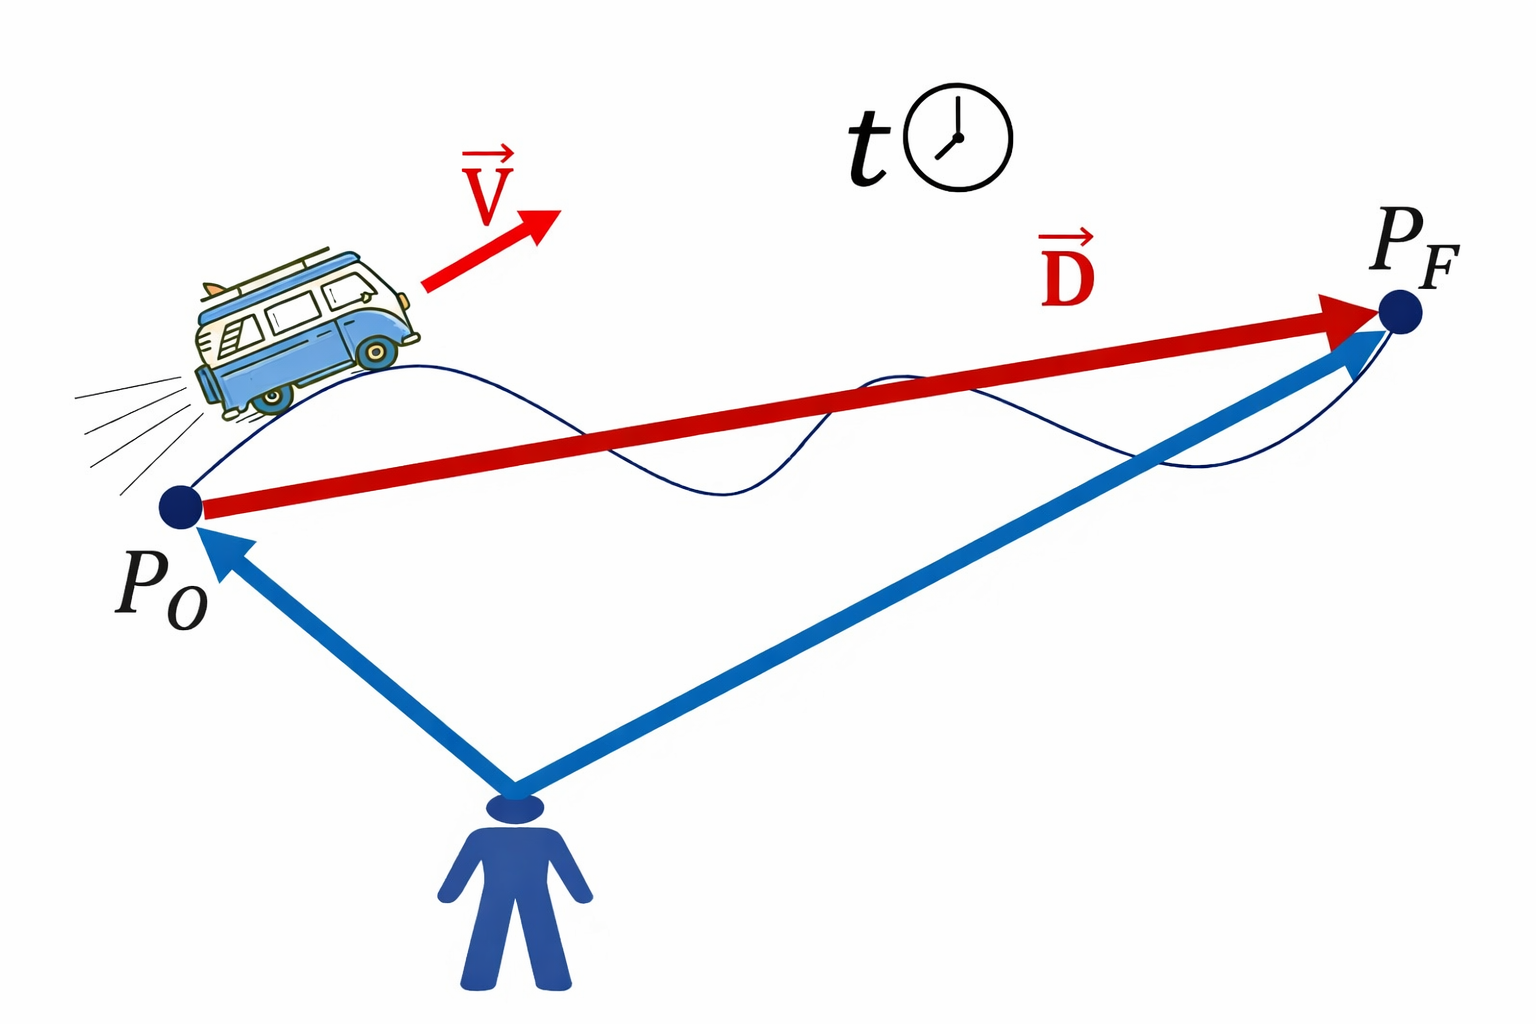
\includegraphics[width=0.6\textwidth]{images/cinematicImages/cinematic.png}
    }
    \caption*{Nota: Representa la relación entre posición y tiempo en el movimiento de un cuerpo.} 
\end{figure}

\vspace{-20pt}

\subsection{Sistema de referencia}
Es el marco o conjunto de coordenadas desde el cual un observador describe la posición y el movimiento de un objeto. Permite establecer medidas de distancia, dirección y tiempo.

\begin{figure}[H]
    \centering
    \captionsetup{width=0.6\textwidth}
    \caption{Sistema de referencia}
    \adjustbox{margin={0pt 10pt 0pt 0pt}}{
        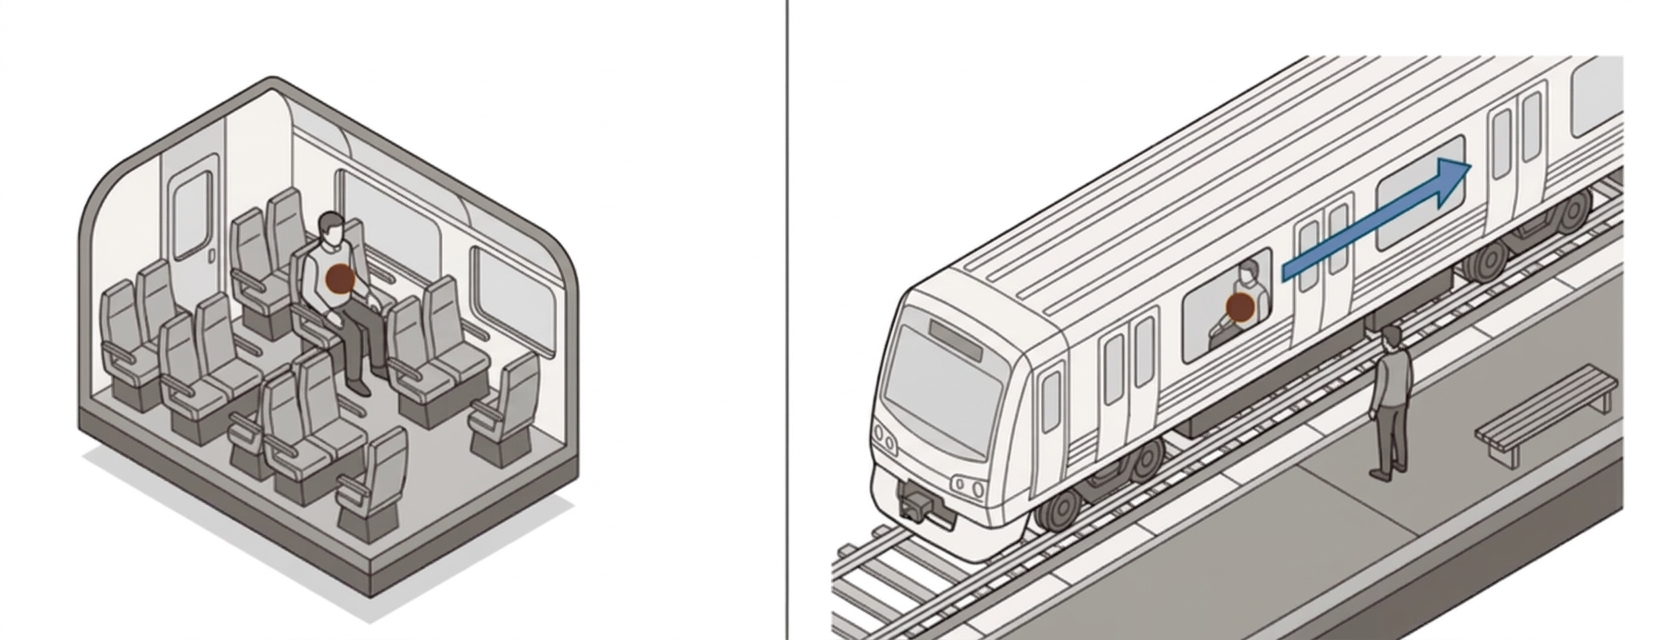
\includegraphics[width=0.7\textwidth]{images/cinematicImages/referenceSystem.png}
    }
    \caption*{Nota: Sistema de referencia desde el observador que describe la posición y el movimiento de un objeto. }
\end{figure}

\vspace{-20pt}

\subsubsection{Observador interno}
Es aquel que se encuentra dentro del sistema en movimiento, es decir, forma parte del cuerpo que se desplaza. Desde su perspectiva, los objetos que se mueven junto a él parecen estar en reposo, mientras que los elementos externos aparentan moverse en sentido contrario.

\subsubsection{Observador externo}
Es aquel que se encuentra fuera del sistema en movimiento, observando el desplazamiento desde un punto fijo. Desde su perspectiva, puede apreciar con claridad la trayectoria, la velocidad y los cambios de posición del cuerpo en movimiento.

\subsection{Posición}
La posición de un objeto indica su ubicación en el espacio respecto a un punto del sistema de referencia (origen). Se representa generalmente con la variable $x$ para el caso unidimensional.

\begin{itemize}
    \item \textbf{En una dimensión (1D):} la posición se describe mediante una sola coordenada, generalmente $x$, que indica la distancia (con signo) respecto al origen.
    \item \textbf{En dos dimensiones (2D):} la posición se describe mediante un vector $\vec{r}$ compuesto por dos coordenadas, $x$ e $y$, que determinan la ubicación del objeto en el plano.
\end{itemize}

\begin{figure}[H]
    \centering
    \captionsetup{width=0.6\textwidth}
    \caption{Posición de un cuerpo en una dimensión}
    \includegraphics[width=0.7\linewidth]{images/cinematicGraphics/1DPosition.jpg}
    \caption*{Nota: Representación de la posición de un cuerpo en un sistema unidimensional. }
\end{figure}

\vspace{-60pt}

\begin{align*}
    \Aboxed{\vec{r} = x_0(\pm \hat{\imath})}
\end{align*}

\begin{figure}[H]
    \centering
    \captionsetup{width=0.6\textwidth}
    \caption{Posición de un cuerpo en dos dimensiones}
    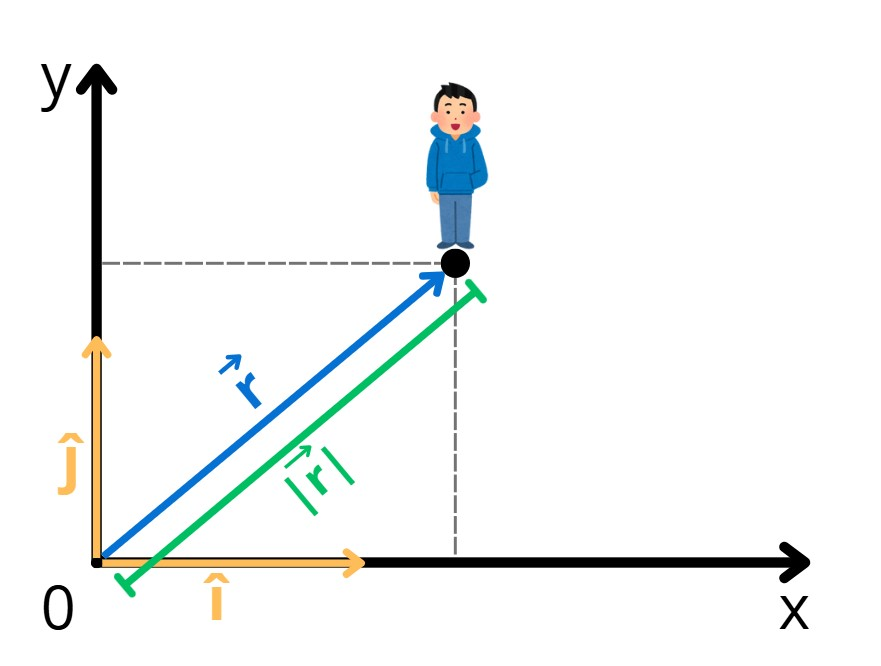
\includegraphics[width=0.7\linewidth]{images/cinematicGraphics/2DPosition.jpg}
    \caption*{Nota: Representación de la posición de un cuerpo en un plano bidimensional. }
\end{figure}

\vspace{-60pt}

\begin{align*}
    \Aboxed{\vec{r} = x\hat{\imath} + y\hat{\jmath}}\\
    \Aboxed{|\vec{r}| = \sqrt{x^2 + y^2}}
\end{align*}

\vspace{-20pt}

\[
[\vec{r}\,] = [\mathrm{m}] \quad \text{S.I.} 
\]

\subsection{Desplazamiento}
El desplazamiento es la variación de posición de un objeto entre dos instantes de tiempo.

\begin{figure}[H]
    \centering
    \captionsetup{width=0.5\textwidth}
    \caption{Desplazamiento en dos dimensiones}
    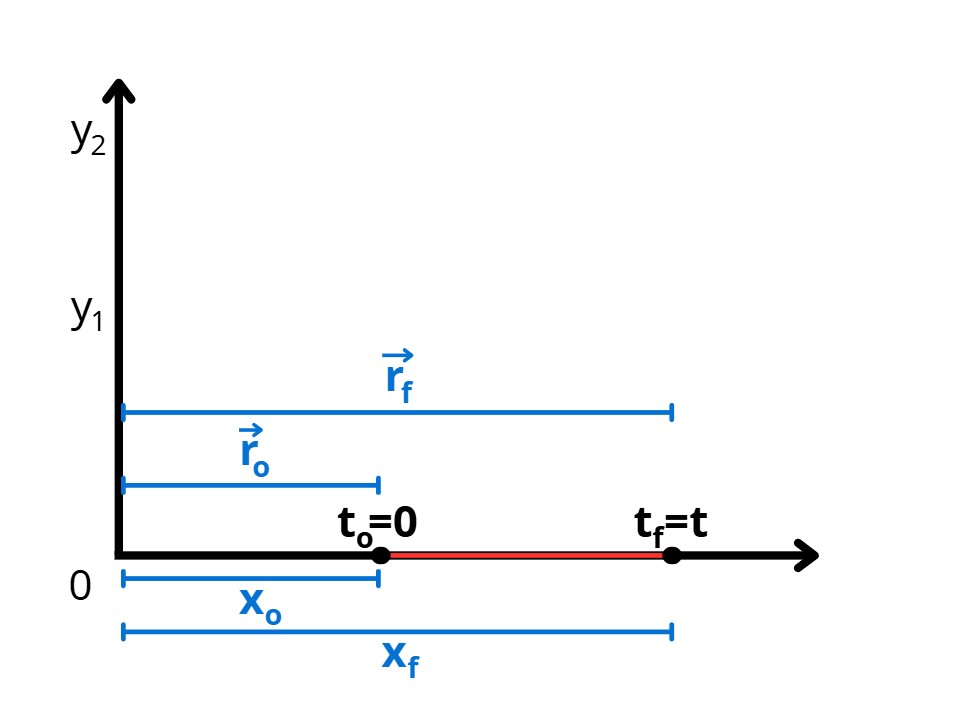
\includegraphics[width=0.7\linewidth]{images/cinematicGraphics/1DDisplacement.jpg}
    \caption*{Nota: Representación del desplazamiento de un cuerpo en un plano bidimensional. }
\end{figure}

\vspace{-60pt}

\begin{align}
    \Aboxed{\Delta \vec{x} = \vec{x}_f - \vec{x}_o}
\end{align}

\begin{figure}[H]
    \centering
    \captionsetup{width=0.5\textwidth}
    \caption{Desplazamiento en dos dimensiones}
    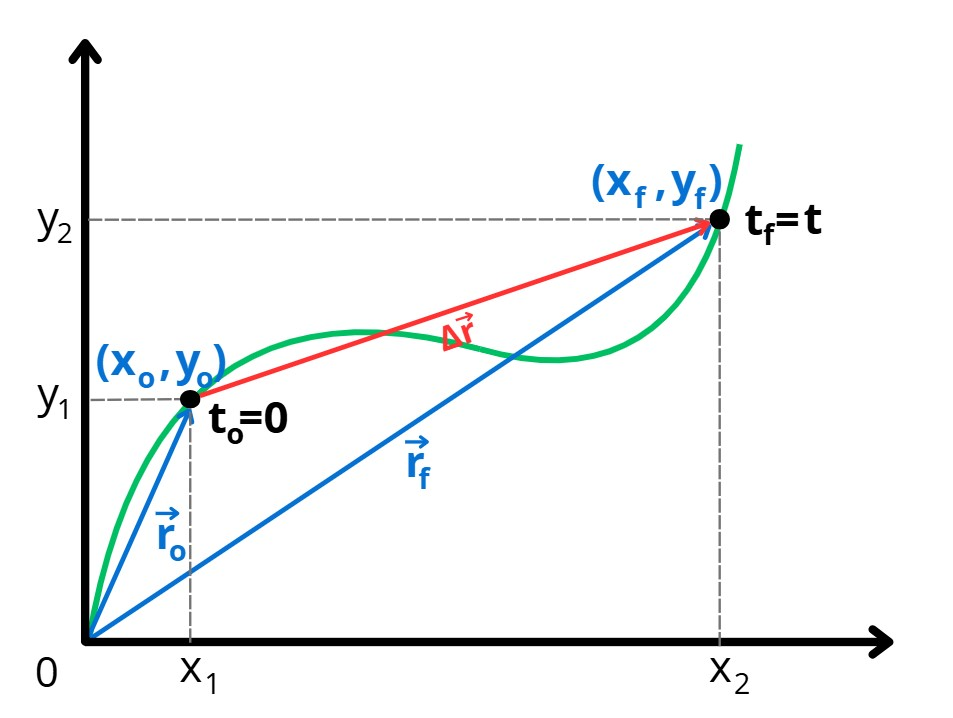
\includegraphics[width=0.7\linewidth]{images/cinematicGraphics/2DDisplacement.jpg}
    \caption*{Nota: Representación del desplazamiento de un cuerpo en un plano bidimensional. }
\end{figure}

\vspace{-60pt}

\begin{align}
    \Aboxed{\Delta \vec{r} = \vec{r}_f - \vec{r}_o}
\end{align}
\begin{align*}
    \vec{r}_o = x_o \hat{\imath} + y_o \hat{\jmath}\\
    \vec{r}_f = x_f \hat{\imath} + y_f \hat{\jmath}
\end{align*}

\vspace{-20pt}

\[
[\Delta \vec{r}\,] = [\mathrm{m}] \quad \text{S.I.} 
\]

Donde $x_f$ es la posición final y $x_0$ es la posición inicial.\\
El desplazamiento puede ser positivo, negativo o cero.

\subsection{Velocidad y rapidez}

\subsubsection{Velocidad}
La velocidad es una magnitud vectorial que expresa la variación de posición por unidad de tiempo. A diferencia de la rapidez, considera la dirección y el sentido del movimiento.

\begin{figure}[H]
    \centering
    \captionsetup{width=0.5\textwidth}
    \caption{Vector velocidad}
    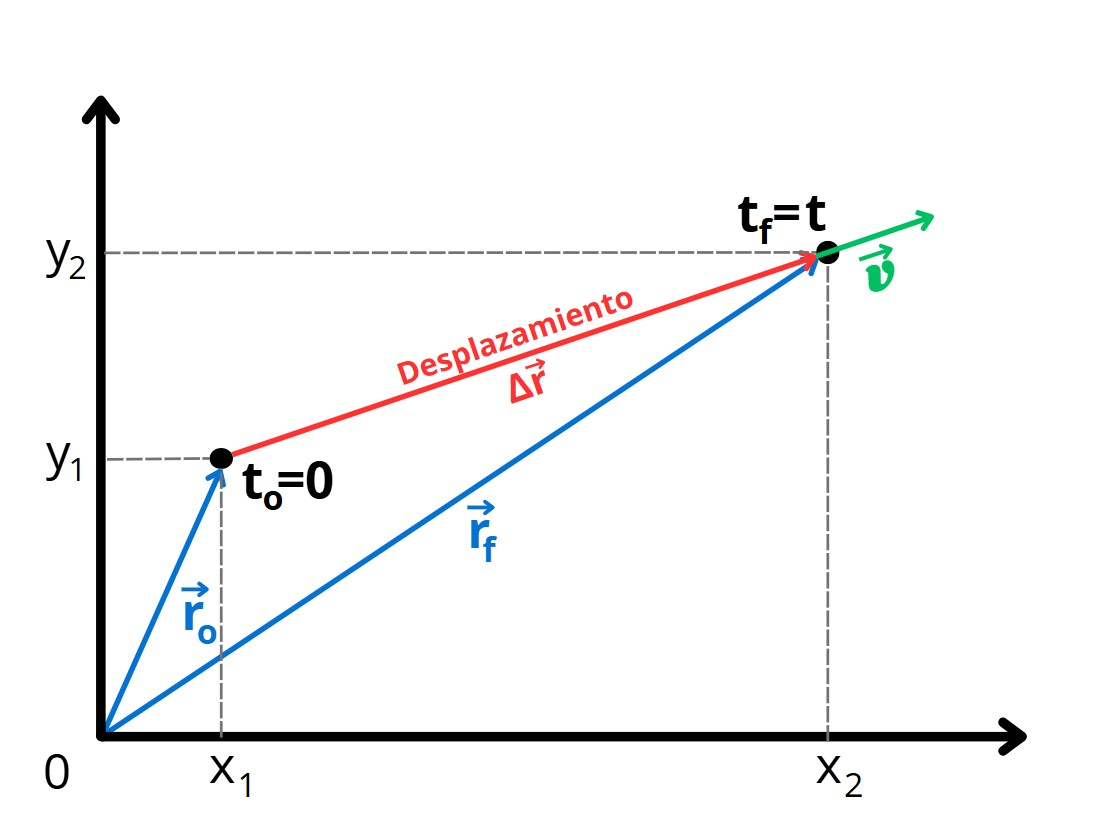
\includegraphics[width=0.5\textwidth]{images/cinematicGraphics/speedV.jpg}
    \caption*{Nota: Representación del vector velocidad, dirección y sentido en el plano.}
\end{figure}

\vspace{-40pt}
\[
\text{velocidad} = \frac{\text{desplazamiento}}{t} = \frac{\Delta{x}}{t}
\]

\vspace{-20pt}

\begin{align*}
    \Aboxed{\displaystyle {v} = \frac{\Delta x}{t}}
\end{align*}

\subsubsection{Rapidez}

La rapidez es una magnitud escalar que indica qué tan rápido se mueve un objeto.

\begin{figure}[H]
    \centering
    \captionsetup{width=0.5\textwidth}
    \caption{Magnitud de la velocidad}
    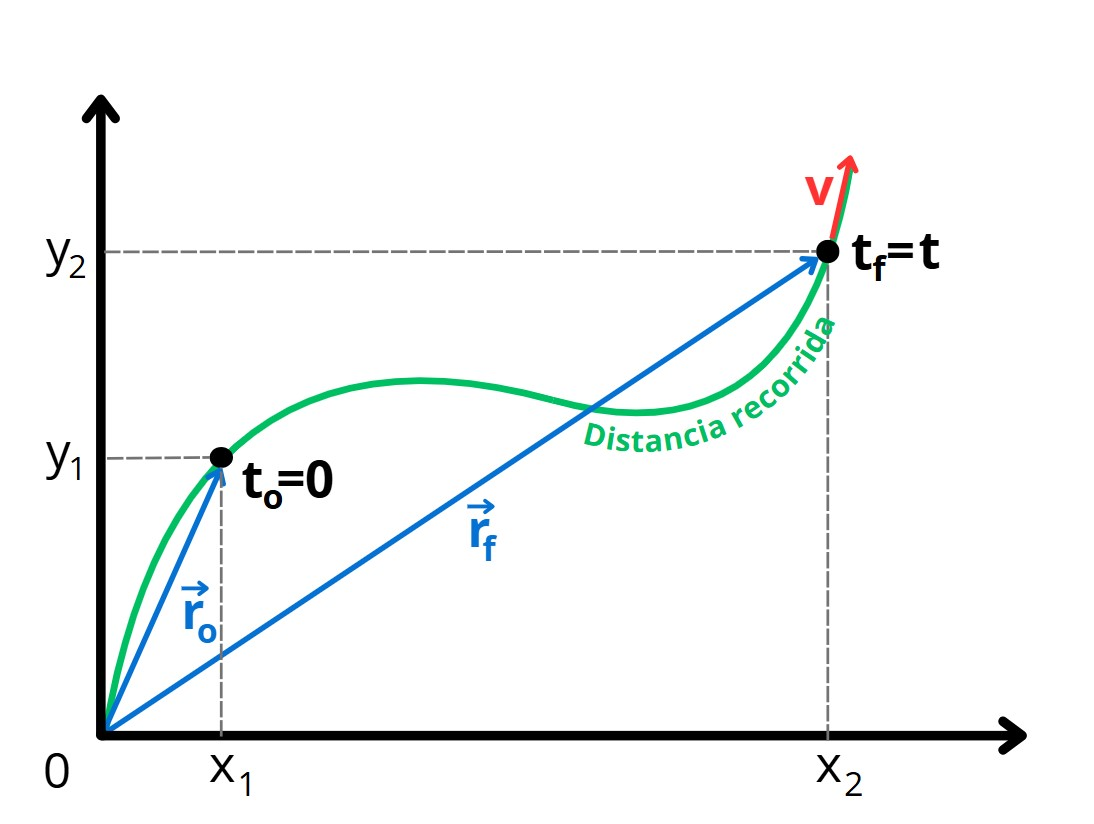
\includegraphics[width=0.5\textwidth]{images/cinematicGraphics/speedR.jpg}
    \caption*{Nota: Representación de la rapidez como el valor escalar de la velocidad}
\end{figure}

\vspace{-40pt}

\[
\text{rapidez} = \frac{\text{distancia recorrida}}{t} = \frac{\text{d}}{t}
\]

\vspace{-20pt}

\begin{align*}
    \Aboxed{\displaystyle \text{v} = \frac{\text{d}}{t}}
\end{align*}

\subsection{Velocidad media e instantánea}

\subsubsection{Velocidad media}
La velocidad media es una magnitud vectorial que se define como el cambio de posición (desplazamiento) dividido entre el intervalo de tiempo en el que ocurre ese cambio.

\begin{figure}[H]
    \captionsetup{width=0.5\textwidth}
    \caption{Velocidad media en un intervalo de tiempo}
    \centering
    \includegraphics[width=0.6\textwidth]{images/cinematicGraphics/averageSpeed.jpg}
    \caption*{Nota: Representación del desplazamiento en un intervalo de tiempo.}
\end{figure}

\vspace{-50pt}

\begin{align}
    \Aboxed{\displaystyle \vec{v}_m = \frac{\Delta \vec{r}}{\Delta t}} = \frac{\vec{r}_f - \vec{r}_o}{\vec{t}_f - \vec{t}_o}
\end{align}

\vspace{-20pt}

\[
[\vec{v}_m\,] = [\frac{m}{s}] \quad \text{S.I.} 
\]

\subsubsection{Velocidad instantánea}
La velocidad instantánea es la velocidad de un objeto en un instante preciso de tiempo. Se obtiene como el límite de la velocidad media cuando el intervalo de tiempo tiende a cero.\\
Este límite es lo que en cálculo se conoce como la derivada de la posición respecto al tiempo.
\begin{figure}[H]
    \centering
    \captionsetup{width=0.5\textwidth}
    \caption{Velocidad instantánea en un punto de la trayectoria}
    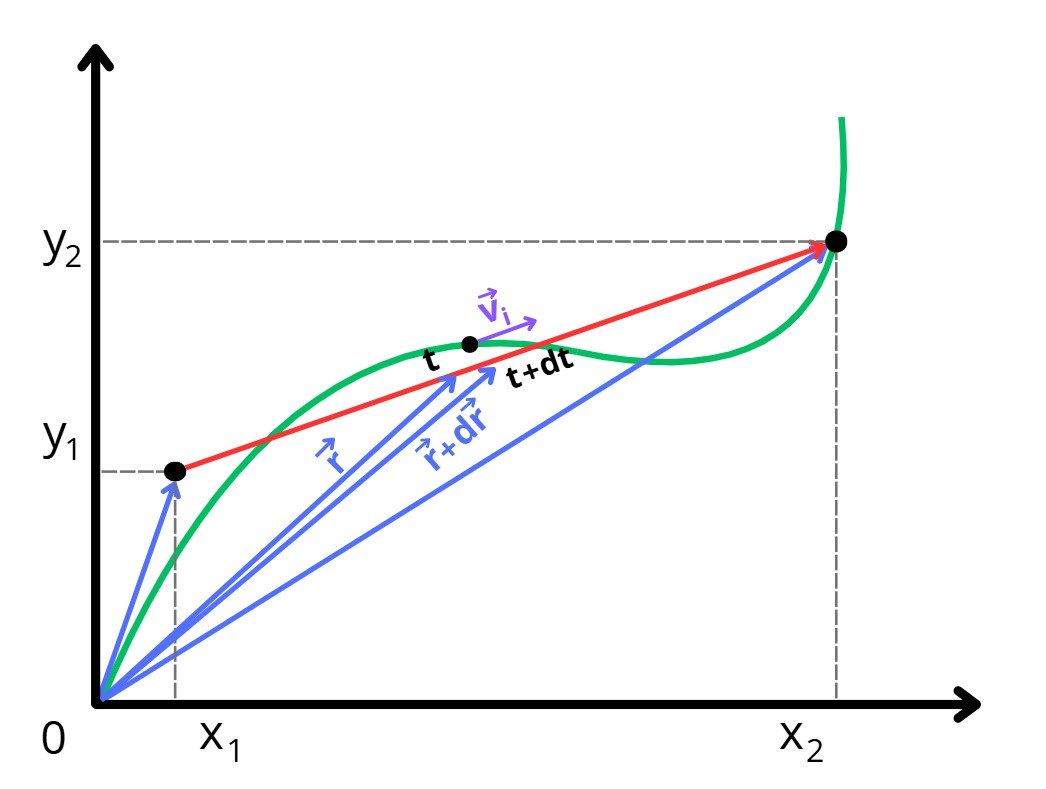
\includegraphics[width=0.6\textwidth]{images/cinematicGraphics/instantSpeed.jpg}
    \caption*{Representación de la velocidad instantánea como la pendiente de la curva posición-tiempo en un punto específico.}
\end{figure}

\vspace{-40pt}

\begin{align}
    \Aboxed{\vec{v} = \lim_{\Delta t \to 0} \frac{\Delta \vec{r}}{\Delta t}} = \frac{d\vec{r}}{dt}
\end{align}

\vspace{-20pt}

\[
[\vec{v}\,] = [\frac{m}{s}] \quad \text{S.I.} 
\]

\subsubsection{Ejemplo}

Determinar la velocidad instantánea de la partícula.

\begin{figure}[H]
    \centering
    \captionsetup{width=0.5\textwidth}
    \caption{Velocidad instantánea en un punto}
    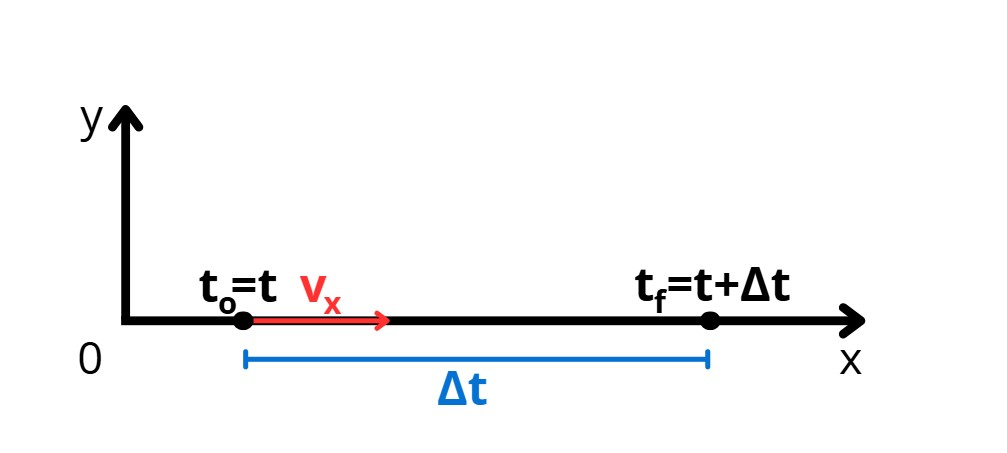
\includegraphics[width=0.6\textwidth]{images/demonstrations/example1.jpg}
    \caption*{Nota: Representación de la velocidad instantánea en un punto de la trayectoria.}
\end{figure}
\vspace{-40pt}

% chktex-file 3
\begin{align*}
&\textbf{Comprobación usando integrales:} \\
    \vec{v_x} &= \lim_{\Delta t \to 0} \frac{\Delta \vec{x}}{\Delta t} \\
    \vec{v_x} &= \lim_{\Delta t \to 0} \frac{x_f(t_f) - x_o(t_o)}{\Delta t} \\
&\text{Considerar } x(t) = t^2: \\    
    v_x &= \lim_{\Delta t \to 0} \frac{t_f^2 - t_o^2}{\Delta t} \\
    v_x &= \lim_{\Delta t \to 0} \frac{(t + \Delta t)^2 - t^2}{\Delta t} \\
    v_x &= \lim_{\Delta t \to 0} \frac{\cancel{t^2} + 2t\Delta t + (\Delta t)^2 - \cancel{t^2}}{\Delta t} \\
    v_x &= \lim_{\Delta t \to 0} \frac{\cancel{\Delta t}(2t + \Delta t)}{\cancel{\Delta t}} \\
    v_x &= \lim_{\Delta t \to 0} (2t + \cancel{\Delta t}) \\
    \Aboxed{v_x &= 2t} \\
\end{align*}
\begin{align*}
&\textbf{Comprobación usando derivada:} \\
    v_x &= \frac{dx(t)}{dt} \\
    v_x &= \frac{d}{dt}(t^2) \\
    v_x &= 2t^{2-1} \\
    \Aboxed{v_x &= 2t}
\end{align*}

\vspace{-30pt}

\[
\Rightarrow \quad \text{Ambos métodos coinciden.}
\]

\subsection{Aceleración media e instantánea}

\begin{figure}[H]
    \centering
    \captionsetup{width=0.5\textwidth}
    \caption{Aceleración media en un intervalo de tiempo}
    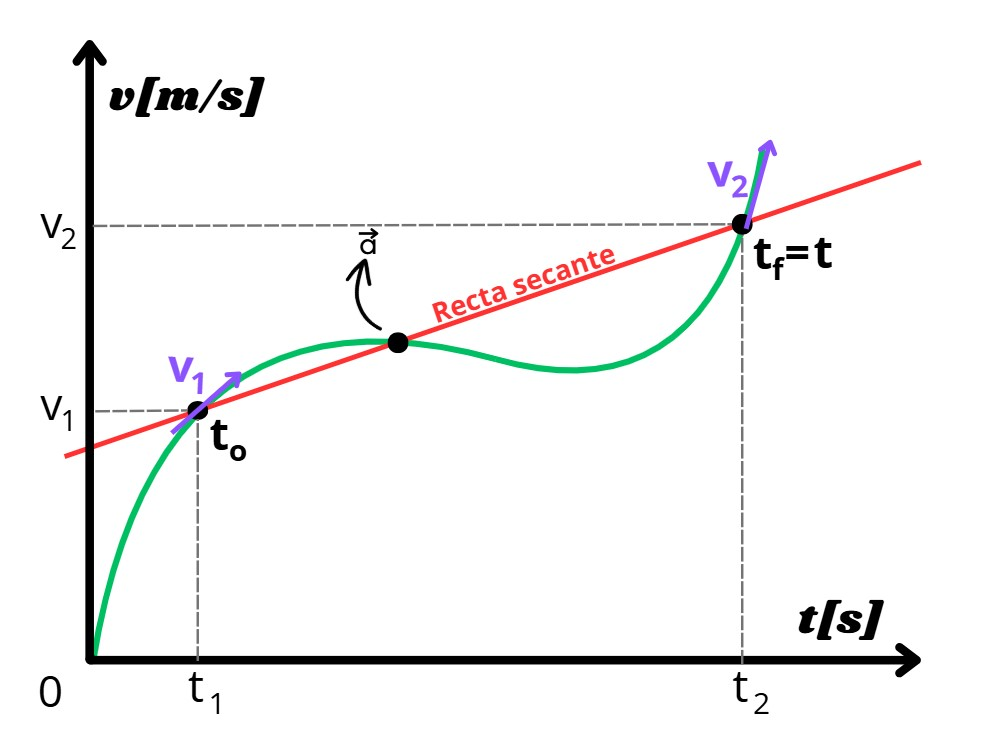
\includegraphics[width=0.6\textwidth]{images/cinematicGraphics/averageAcceleration.jpg}
    \caption*{Representación de la aceleración como cambio de la velocidad en el tiempo.}
\end{figure}

\vspace{-40pt}

\[
[a] = [\frac{m/s}{s}] = [\frac{m}{s^2}]  \quad \text{S.I.} 
\]

\subsubsection{Aceleración media}
La aceleración media mide la variación de la velocidad en un intervalo de tiempo determinado:
\vspace{-20pt}

\begin{align}
    \Aboxed{\displaystyle \vec{a}_m = \frac{\Delta \vec{v}}{\Delta t}} = \frac{v_f - v_0}{t_f - t_0}
\end{align}

\subsubsection{Aceleración instantánea}

La aceleración instantánea es la aceleración de un objeto en un instante preciso. Se define como el límite de la aceleración media cuando el intervalo de tiempo tiende a cero:
\vspace{-20pt}

\begin{align}
\Aboxed{\vec{a} &= \lim_{\Delta t \to 0} (\frac{\Delta v}{\Delta t})}
\end{align}

\begin{align*}
\vec{a} &= \frac{\Delta v}{\Delta t}(t) \\
\vec{a} &= \frac{d\vec{v}}{dt} \\
\vec{v} &= v_x \hat{\imath} + v_y \hat{\jmath} + v_z \hat{k} \\
\vec{a} &= \frac{d}{dt}(v_x \hat{\imath} + v_y \hat{\jmath} + v_z \hat{k}) \\
\vec{a} &= (\frac{dv_x}{dt})\hat{\imath} + (\frac{dv_y}{dt})\hat{\jmath} + (\frac{dv_z}{dt})\hat{k}
\end{align*}

\vspace{-10pt}

\begin{align*}
a_x &= \frac{dv_x}{dt}, \quad
a_y = \frac{dv_y}{dt}, \quad
a_z = \frac{dv_z}{dt}\\
\vec{a} &= a_x \hat{\imath} + a_y \hat{\jmath} + a_z \hat{k}\\
\end{align*}
\vspace{-40pt}
\begin{align}
    \Aboxed{|\vec{a}| &= a = \sqrt{a_x^2 + a_y^2 + a_z^2}}
\end{align}

Geométricamente, corresponde a la pendiente de la recta tangente a la curva velocidad-tiempo en un punto dado.

\subsubsection{Ejemplo 2}

Determinación de la aceleración usando la definición de aceleración instantánea.

\begin{figure}[H]
    \centering
    \captionsetup{width=0.5\textwidth}
    \caption{Aceleración instantánea en función del tiempo}
    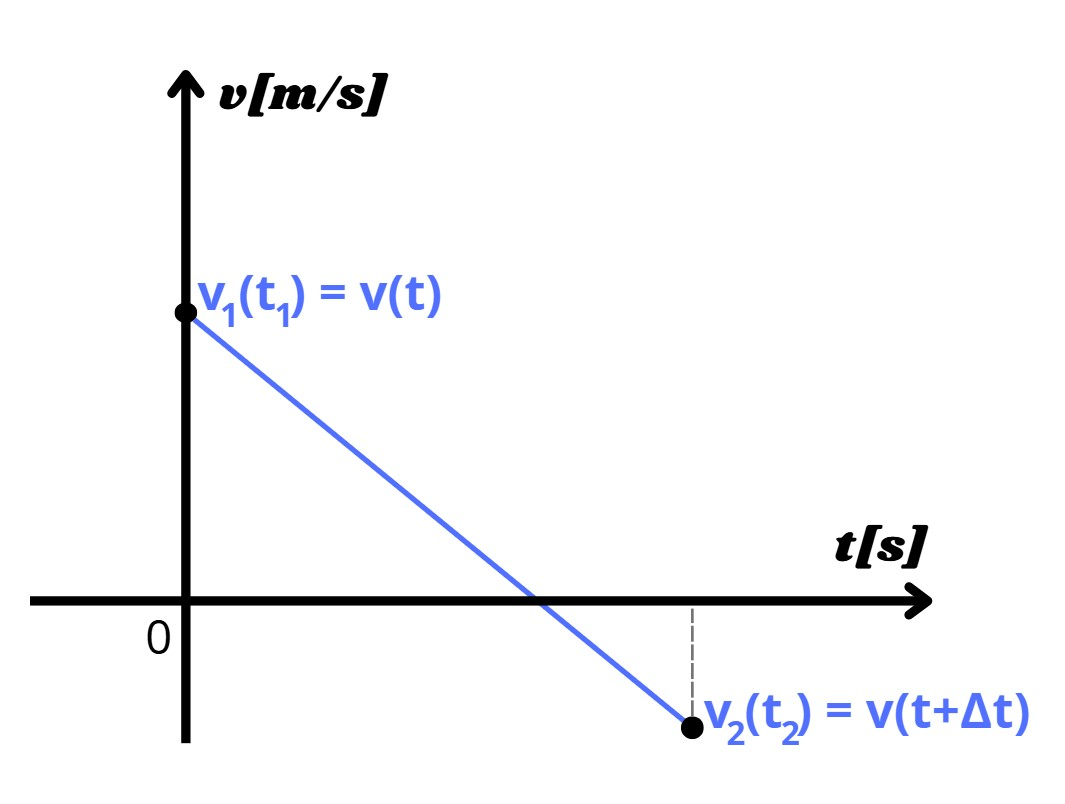
\includegraphics[width=0.6\textwidth]{images/demonstrations/example2.jpg}
    \caption*{Nota: Representación de la aceleración obtenida como derivada de la velocidad respecto al tiempo. }
\end{figure}

\begin{align*}
&\textbf{Comprobación usando integrales:} \\
    a_y &= \lim_{\Delta t \to 0} \frac{v_y(t+\Delta t) - v_y(t)}{\Delta t}
    \quad \text{con } v_{0y}=\text{ctte},\; g=9.8\,\text{m/s}^2 \\
    a_y &= \lim_{\Delta t \to 0} \left(\frac{\Delta v}{\Delta t}\right) \\
    a_y &= \lim_{\Delta t \to 0} \left(\frac{v(t_2) - v(t_1)}{\Delta t}\right) \\
    a_y &= \lim_{\Delta t \to 0} \left(\frac{(v_{0y} - gt_2)-(v_{0y} - gt_1)}{\Delta t}\right) \\
    a_y &= \lim_{\Delta t \to 0} \frac{[v_{0y} - g(t+\Delta t)] - [v_{0y} - gt]}{\Delta t} \\
    a_y &= \lim_{\Delta t \to 0} \frac{\cancel{v_{0y}} - \cancel{gt} - g\Delta t - \cancel{v_{0y}} + \cancel{gt}}{\Delta t} \\
    a_y &= \lim_{\Delta t \to 0} \frac{-g\cancel{\Delta t}}{\cancel{\Delta t}} \\
    a_y &= \lim_{\Delta t \to 0} (-g) \\
    \Aboxed{a_y &= -g} \\
&\textbf{Comprobación usando derivada:} \\
    \vec{a} &= \frac{dv(t)}{dt} \\
    \vec{a} &= \frac{d}{dt}(v_{0y}-gt) \\
    \vec{a} &= \frac{d}{dt}(\cancel{v_{0y}}) - \frac{d}{dt}(gt)\\
    \vec{a} &= -g \cancel{\frac{dt}{dt}}\\
    \Aboxed{a &= -g}
\end{align*}
